\documentclass{article}


% if you need to pass options to natbib, use, e.g.:
%     \PassOptionsToPackage{numbers, compress}{natbib}
\PassOptionsToPackage{sort, numbers, compress}{natbib}
% before loading neurips_2022


% ready for submission
% \usepackage{neurips_2024}


% to compile a preprint version, e.g., for submission to arXiv, add add the
% [preprint] option:
%     \usepackage[preprint]{neurips_2022}


% to compile a camera-ready version, add the [final] option, e.g.:
     \usepackage[final]{neurips_2024}


% to avoid loading the natbib package, add option nonatbib:
%    \usepackage[nonatbib]{neurips_2022}


\usepackage[utf8]{inputenc} % allow utf-8 input
\usepackage[T1]{fontenc}    % use 8-bit T1 fonts
%\usepackage{hyperref}       % hyperlinks
\usepackage{url}            % simple URL typesetting
\usepackage{booktabs}       % professional-quality tables
\usepackage{amsfonts}       % blackboard math symbols
\usepackage{nicefrac}       % compact symbols for 1/2, etc.
\usepackage{microtype}      % microtypography
\usepackage{xcolor}         % colors


\usepackage{makeidx}
\usepackage{amsmath,amsfonts,amssymb,amsthm}
\usepackage{graphics}
\usepackage{graphicx}
\allowdisplaybreaks
\thispagestyle{empty}
\usepackage{framed}

\usepackage{subfigure}

\usepackage{framed}
\usepackage{mathrsfs}
\usepackage{enumerate}
\usepackage{tikz}
\usetikzlibrary{matrix}
\usepackage[all]{xy}
\usetikzlibrary{shapes}
\usetikzlibrary{decorations.markings}
%\usepackage{hyperref}
\usepackage{multirow}
\usepackage{bm}

\definecolor{mydarkblue}{rgb}{0,0.08,0.45}
\usepackage[colorlinks=true,
    linkcolor=mydarkblue,
    citecolor=mydarkblue,
    filecolor=mydarkblue,
    urlcolor=mydarkblue,
    pdfview=FitH]{hyperref}

\usepackage[T1]{fontenc}

% Tim's Commands
\newcommand{\cA}{\mathcal A}
\newcommand{\cB}{\mathcal B}
\newcommand{\cC}{\mathcal C}
\newcommand{\cD}{\mathcal D}
\newcommand{\cE}{\mathcal E}
\newcommand{\cP}{\mathcal P}
\newcommand{\cS}{\mathcal S}
\newcommand{\cT}{\mathcal T}
\newcommand{\cL}{\mathcal L}
\newcommand{\K}{\mathbb K}
\newcommand{\N}{\mathbb N}
\newcommand{\Z}{\mathbb Z}
\newcommand{\R}{\mathbb R}
\newcommand{\Q}{\mathbb Q}

%\newcommand{\max}{\operatornamewithlimits{\mbox{argmax}\,}}

\newcommand{\Aff}{\mathrm{Aff}\,}
\newcommand{\Abb}{{\textrm Abb}}

\newcommand{\adj}{{\textrm adj}\;}
\newcommand{\aff}{\mathrm{aff}\,}
\newcommand{\Def}{\mathrm{def}\;}
\newcommand{\End}{\mathrm{End}}

\newcommand{\Aut}{\mathrm{Aut}}
\newcommand{\GL}{\text{GL}}

\newcommand{\Hom}{\textrm Hom}





\newcommand{\bS}{\mathbb{S}}
\newcommand{\Sn}{\bS^n}




\newcommand{\bE}{\mathbb E}

\newcommand{\cN}{\mathcal N}

\newcommand{\B}{\mathbb B}
\newcommand{\bB}{\mathbb B}
%\newcommand{\C}{\mathbb C}

\newtheorem{proposition}{Proposition}[section]
\newtheorem{theorem}{Theorem}[section]
\newtheorem{lemma}{Lemma}[section]

\def\argmin{ \mathrm{argmin}}

\def\argmax{ \mathrm{argmax}}

\newcommand{\bd}{\mathrm{bd}\,}
\newcommand{\bi}{\binom}
\newcommand{\Char}{\mathrm{char}}
\newcommand{\cone}{\mathrm{cone}\;}
\newcommand{\co}{\mathrm{conv}\,}
\newcommand{\core}{\mathrm{core}\,}
\newcommand{\cl}{\mathrm{cl}\,}
\newcommand{\clco}{\overline{\mathrm{conv}}\,}
\newcommand{\diag}{\mathrm{diag}\,}
\newcommand{\dist}{\mathrm{dist}\,}
\newcommand{\dom}{\mathrm{dom}\,}
\newcommand{\conjug}{\;\overset{*}{\longleftrightarrow }\;}
\newcommand{\epi}{\mathrm{epi}\,}
\newcommand{\ext}{\mathrm{ext}\,}
\def\elim{{\textrm e-}\hspace{-0.5pt}\lim}
\def\glim{{\textrm g-}\hspace{-0.5pt}\lim}
\newcommand{\gph}{\mathrm{gph}\,}
\newcommand{\grad}{\mathrm{grad}\;}
\newcommand{\id}{\mathrm{id}\,}
\newcommand{\ip}[1]{\left\langle #1 \right\rangle}
\newcommand{\ind}{\mathrm{Ind}\,}
\newcommand{\inter}{\mathrm{int}\,}
\newcommand{\im}{\mathrm{rge}\,}
\newcommand{\Ima}{\mathrm{Im}}
\newcommand{\lev}{\mathrm{lev}}
\def\Lim{\mathop{{\textrm Lim}\,}}
\def\Liminf{\mathop{{\textrm Lim}\,{\textrm inf}}}
\def\Limsup{\mathop{{\textrm Lim}\,{\textrm sup}}}
\newcommand{\nul}{\mathrm{nul}\,}
\newcommand{\p}{\partial}
\newcommand{\rge}{\mathrm{rge}\,}

\newcommand{\rank}{\mathrm{rank}\,}

\newcommand{\Real}{\mathrm{Re}}
\newcommand{\sgn}{\mathrm{sgn}?}
\newcommand{\rbar}{\overline{\mathbb R}}
\newcommand{\rp}{\mathbb R\cup \{+\infty\}}
\newcommand{\rbd}{\mathrm{rbd}\,}
\newcommand{\ri}{\mathrm{ri}\,}
\newcommand{\set}[2]{\left\{#1\,\left\vert\; #2\right.\right\}}

\newcommand{\Uni}{\mathrm{U}}
\newcommand{\Orth}{\mathrm{O}}
\newcommand{\SU}{\mathrm{SU}}
\newcommand{\SO}{\mathrm{SO}}

\newcommand{\spn}{\mathrm{span}\,}

\newcommand{\Sym}{\mathrm{Sym}\,}

\newcommand{\tr}{\mathrm{tr}\,}

\newcommand{\lin}{\mathrm{span}\,}

\newcommand{\AND}{\quad\mbox{and}\quad}
\newcommand{\IFF}{\quad\Longleftrightarrow\quad}

% definition of Cartesian products
\def\XX{\operatornamewithlimits{\mbox{\sf\large X}}}
\def\XXX{\operatornamewithlimits{\mbox{\sf\Large X}}}

\pagestyle{empty}

\usepackage[algoruled, linesnumbered, shortend, lined]{algorithm2e}
\usepackage{algpseudocode}

\SetAlgoSkip{bigskip}
\SetKwInput{Input}{Input\hspace{34pt}{ }}
\SetKwInput{Output}{Output\hspace{27pt}{ }}
\SetKwInput{Initialize}{Initialize\hspace{20pt}{ }}
\SetKwInput{Parameters}{Parameters\hspace{2pt}{ }}

\newcommand{\prox}{\text{prox}}

\title{Project Report - Image Deblurring}


% The \author macro works with any number of authors. There are two commands
% used to separate the names and addresses of multiple authors: \And and \AND.
%
% Using \And between authors leaves it to LaTeX to determine where to break the
% lines. Using \AND forces a line break at that point. So, if LaTeX puts 3 of 4
% authors names on the first line, and the last on the second line, try using
% \AND instead of \And before the third author name.


\author{%
  Alexander Kakabadze \\
  Student ID: 123456789
  % examples of more authors
  \And
  Edmand Yu \\
  Student ID: 123456789\\
 \AND
 Lilian Yuan\\
 Student ID: 123456789\\
 \And
 Rahul Padmanabhan\\
 Student ID: 567894321\\ 
}

% Math macros to be imported into main.tex

%ELLIOT
\def\N{\mathbb{N}}
\def\R{\mathbb{R}}
\def\Filt{\mathscr{F}}
\renewcommand\ss{{\boldsymbol s}}
\renewcommand\gg{{\boldsymbol g}}

%KIWON
\def\aa{{\boldsymbol a}}
\def\bb{{\boldsymbol b}}
\def\hh{{\boldsymbol h}}

%COURTNEY
\def\xx{{\boldsymbol x}}
\def\qq{{\boldsymbol q}}
\def\dd{{\boldsymbol d}}
\def\XX{{\boldsymbol X}}
\def\YY{{\boldsymbol Y}}
\def\ZZ{{\boldsymbol Z}}
\def\aa{{\boldsymbol a}}
\def\bb{{\boldsymbol b}}
\def\rr{{\boldsymbol r}}
\def\ee{{\boldsymbol e}}
\def\cc{{\boldsymbol c}}
\def\qq{{\boldsymbol q}}
\def\vv{{\boldsymbol v}}

\def\WW{{\boldsymbol W}}
\def\JJ{{\boldsymbol J}}
\def\KK{{\boldsymbol K}}
\def\II{{\text{\textbf{I}}}}
\def\yy{{\boldsymbol y}}
\def\vv{{\boldsymbol v}}
\def\uu{{\boldsymbol u}}
\def\ww{{\boldsymbol w}}
\def\zz{{\boldsymbol z}}
\def\SS{{\boldsymbol S}}
\def\BB{{\boldsymbol B}}
\def\AA{{\boldsymbol A}}
\def\CC{{\boldsymbol C}}
\def\FF{{\boldsymbol F}}
\def\GG{{\boldsymbol G}}
\def\MM{{\boldsymbol M}}
\def\DD{{\boldsymbol D}}
\def\OO{{\boldsymbol O}}
\def\PP{{\boldsymbol P}}
\def\TT{{\boldsymbol T}}
\def\bphi{{\boldsymbol \phi}}
\def\QQ{{\boldsymbol Q}}
\def\UU{{\boldsymbol U}}
\def\VV{{\boldsymbol V}}
\def\HH{{\boldsymbol H}}
\def\balpha{{\boldsymbol \alpha}}
\def\bpsi{{\boldsymbol \psi}}
\def\LLambda{{\boldsymbol \Lambda}}
\def\xxi{  {\boldsymbol \xi} } 
\def\SSigma{{\boldsymbol \Sigma}}

\def\YY{ {\boldsymbol Y} }

\def\nnu{{\boldsymbol \nu}}
\def\eeps{{\boldsymbol \varepsilon}}
\def\eeta{{\boldsymbol \eta}}
\def\DDelta{{\boldsymbol \Delta}}
\def\llambda{{\boldsymbol \lambda}}
\def\bbeta{{\boldsymbol \beta}}

\def\g{{g}}

\def\dif{\mathop{}\!\mathrm{d}}
\def\Proba{\mathbb{P}}
\def\MP{\mu_{\mathrm{MP}}}
\def\RR{{\widehat{\bm {R}}}}
\def\EE{{\mathbb E}\,}
%\newcommand{\Econd}{\mathbf{E}}
\renewcommand{\vec}{\mathbf{vec}}
%\DeclareMathOperator{\prox}{\mathbf{prox}}

%\DeclareMathOperator*{\argmin}{{arg\,min}}

%\DeclareMathOperator{\tr}{tr}
\def\defas{\stackrel{\text{def}}{=}}
%\DeclareMathOperator*{\dom}{dom}
%\DeclareMathOperator*{\supp}{supp}
%\DeclareMathOperator*{\Fix}{Fix}
%\DeclareMathOperator*{\Var}{Var}
%\DeclareMathOperator*{\argmax}{{arg\,max}}
%\DeclareMathOperator*{\argmin}{{arg\,min}}
%\DeclareMathOperator*{\minimize}{minimize}
%\DeclareMathOperator*{\diag}{\mathbf{diag}}
\DeclareMathOperator*{\ospan}{span}
\def\concentration{\! \! \underset{d \rightarrow \infty}{\mathcal{E}} \!  [\|\nabla f(\xx_{k})\|^2]\,}


\newcommand{\D}{\tilde{D}}
%\newcommand{\B}{\tilde{B}}
\newcommand{\M}{\tilde{M}}
%\newcommand{\K}{\tilde{K}}
%\newcommand{\Z}{\mathcal{Z}}
\newcommand{\W}{\mathcal{W}}
\DeclareMathOperator{\E}{\mathbb{E}}

\newcommand{\Id}{\text{\textbf{I}}}
\DeclareMathOperator{\Exp}{\mathbb{E}}

%\newcommand{\blue}{\color{blue}}



%BEN
\DeclareMathOperator{\ntr}{\bar{tr}}
\newcommand{\gcal}{R}
\newcommand{\gcaltil}{\tilde{R}}
\newcommand{\gcalm}[1]{R^{(#1)}}
\newcommand{\gcaltilm}[1]{\tilde{R}^{(#1)}}
\newcommand{\deq}{\mathrel{\mathop:}=} 


% shortcut for inline equations and alignments
%\newcommand{\eq}[1]{\begin{equation}#1\end{equation}}
%\newcommand{\eqs}[1]{\begin{equation*}#1\end{equation*}}
\newcommand{\al}[1]{\begin{align}#1\end{align}}
\newcommand{\als}[1]{\begin{align*}#1\end{align*}}
\newcommand{\ca}[1]{\begin{cases}#1\end{cases}}

% ( round parentheses )
\newcommand{\pb}[1]{\bigl({#1}\bigr)}
\newcommand{\pB}[1]{\Bigl({#1}\Bigr)}
\newcommand{\pbb}[1]{\biggl({#1}\biggr)}
\newcommand{\pBB}[1]{\Biggl({#1}\Biggr)}
\newcommand{\pa}[1]{\left({#1}\right)}

% [ square brackets ]
\newcommand{\q}[1]{[{#1}]}
\newcommand{\qb}[1]{\bigl[{#1}\bigr]}
\newcommand{\qB}[1]{\Bigl[{#1}\Bigr]}
\newcommand{\qbb}[1]{\biggl[{#1}\biggr]}
\newcommand{\qBB}[1]{\Biggl[{#1}\Biggr]}
\newcommand{\qa}[1]{\left[{#1}\right]}

% { curly braces }
\newcommand{\h}[1]{\{{#1}\}}
\newcommand{\hb}[1]{\bigl\{{#1}\bigr\}}
\newcommand{\hB}[1]{\Bigl\{{#1}\Bigr\}}
\newcommand{\hbb}[1]{\biggl\{{#1}\biggr\}}
\newcommand{\hBB}[1]{\Biggl\{{#1}\Biggr\}}
\newcommand{\ha}[1]{\left\{{#1}\right\}}

% | absolute value |
\newcommand{\abs}[1]{\lvert #1 \rvert}
\newcommand{\absb}[1]{\bigl\lvert #1 \bigr\rvert}
\newcommand{\absB}[1]{\Bigl\lvert #1 \Bigr\rvert}
\newcommand{\absbb}[1]{\biggl\lvert #1 \biggr\rvert}
\newcommand{\absBB}[1]{\Biggl\lvert #1 \Biggr\rvert}
\newcommand{\absa}[1]{\left\lvert #1 \right\rvert}

% || norm ||
\newcommand{\norm}[1]{\lVert #1 \rVert}
\newcommand{\normb}[1]{\bigl\lVert #1 \bigr\rVert}
\newcommand{\normB}[1]{\Bigl\lVert #1 \Bigr\rVert}
\newcommand{\normbb}[1]{\biggl\lVert #1 \biggr\rVert}
\newcommand{\normBB}[1]{\Biggl\lVert #1 \Biggr\rVert}
\newcommand{\norma}[1]{\left\lVert #1 \right\rVert}

\newcommand{\vertiii}[1]{{\left\vert\kern-0.25ex\left\vert\kern-0.25ex\left\vert #1 
    \right\vert\kern-0.25ex\right\vert\kern-0.25ex\right\vert}}
    
\newcommand{\gf}{\bm{\mathscr{X}}^{\text{gf}}}

\newcommand{\sgf}{\bm{\mathscr{X}}^{\text{s-gf}}}

\newcommand{\gd}{\bm{\xx}^{\text{gd}}}

\newcommand{\sgd}{\bm{\xx}^{\text{sgd}}}

\newcommand{\mgd}{\bm{x}^{\text{m-gd}}}

\begin{document}

\maketitle


\begin{abstract}
  This project implements and compares several convex optimization algorithms for image deblurring and denoising.
  We present four different algorithms: Primal Douglas-Rachford Splitting (Spingarn's Method), Primal-Dual Douglas-Rachford Splitting, the alternating direction method of multipliers (ADMM) and the Chambolle-Pock Algorithm.
  Each method is implemented with consideration of computational efficiency and convergence properties.
  The algorithms handle various types of blur kernels, including Gaussian and motion blur, while incorporating different regularization terms such as L1, L2, and isotropic norms.
  Our implementation leverages modern computational tools including PyTorch for efficient tensor operations and automatic differentiation.
  The project includes tests to evaluate the performance of each algorithm in terms of convergence speed, image quality metrics, and computational efficiency.
  The results demonstrate the effectiveness of these convex optimization approaches in restoring degraded images while preserving important image features and textures.
\end{abstract}


\section{Submission of papers to NeurIPS 2024 and Math 463/563}


Please read the instructions below carefully and follow them faithfully.


\subsection{Style}


Papers to be submitted to Math 463/563 must be prepared according to the
instructions presented here. Papers may only be up to {\bf 15} pages long,
including figures. Additional pages \emph{containing only acknowledgments and
references} are allowed. Papers that exceed the page limit will not be
reviewed, or in any other way considered for presentation at the conference.


The margins in 2024 are the same as those in previous years.


Authors are required to use the NeurIPS \LaTeX{} style files obtainable at the
NeurIPS website as indicated below. Please make sure you use the current files
and not previous versions. Tweaking the style files may be grounds for
rejection.


\subsection{Retrieval of style files}


The style files for NeurIPS and other conference information are available on
the World Wide Web at
\begin{center}
  \url{http://www.neurips.cc/}
\end{center}
The file \verb+neurips_2024.pdf+ contains these instructions and illustrates the
various formatting requirements your NeurIPS paper must satisfy.


The only supported style file for NeurIPS 2024 is \verb+neurips_2024.sty+,
rewritten for \LaTeXe{}.  \textbf{Previous style files for \LaTeX{} 2.09,
  Microsoft Word, and RTF are no longer supported!}


The \LaTeX{} style file contains three optional arguments: \verb+final+, which
creates a camera-ready copy, \verb+preprint+, which creates a preprint for
submission to, e.g., arXiv, and \verb+nonatbib+, which will not load the
\verb+natbib+ package for you in case of package clash.


\paragraph{Preprint option}
If you wish to post a preprint of your work online, e.g., on arXiv, using the
NeurIPS style, please use the \verb+preprint+ option. This will create a
nonanonymized version of your work with the text ``Preprint. Work in progress.''
in the footer. This version may be distributed as you see fit. Please \textbf{do
  not} use the \verb+final+ option, which should \textbf{only} be used for
papers accepted to NeurIPS.


At submission time, please omit the \verb+final+ and \verb+preprint+
options. This will anonymize your submission and add line numbers to aid
review. Please do \emph{not} refer to these line numbers in your paper as they
will be removed during generation of camera-ready copies.


The file \verb+neurips_2024.tex+ may be used as a ``shell'' for writing your
paper. All you have to do is replace the author, title, abstract, and text of
the paper with your own.


The formatting instructions contained in these style files are summarized in
Sections \ref{gen_inst}, \ref{headings}, and \ref{others} below.


\section{General formatting instructions}
\label{gen_inst}


The text must be confined within a rectangle 5.5~inches (33~picas) wide and
9~inches (54~picas) long. The left margin is 1.5~inch (9~picas).  Use 10~point
type with a vertical spacing (leading) of 11~points.  Times New Roman is the
preferred typeface throughout, and will be selected for you by default.
Paragraphs are separated by \nicefrac{1}{2}~line space (5.5 points), with no
indentation.


The paper title should be 17~point, initial caps/lower case, bold, centered
between two horizontal rules. The top rule should be 4~points thick and the
bottom rule should be 1~point thick. Allow \nicefrac{1}{4}~inch space above and
below the title to rules. All pages should start at 1~inch (6~picas) from the
top of the page.


For the final version, authors' names are set in boldface, and each name is
centered above the corresponding address. The lead author's name is to be listed
first (left-most), and the co-authors' names (if different address) are set to
follow. If there is only one co-author, list both author and co-author side by
side.


Please pay special attention to the instructions in Section \ref{others}
regarding figures, tables, acknowledgments, and references.


\section{Headings: first level}
\label{headings}


All headings should be lower case (except for first word and proper nouns),
flush left, and bold.


First-level headings should be in 12-point type.


\subsection{Headings: second level}


Second-level headings should be in 10-point type.


\subsubsection{Headings: third level}


Third-level headings should be in 10-point type.


\paragraph{Paragraphs}


There is also a \verb+\paragraph+ command available, which sets the heading in
bold, flush left, and inline with the text, with the heading followed by 1\,em
of space.


\section{Citations, figures, tables, references}
\label{others}


These instructions apply to everyone.


\subsection{Citations within the text}


The \verb+natbib+ package will be loaded for you by default.  Citations may be
author/year or numeric, as long as you maintain internal consistency.  As to the
format of the references themselves, any style is acceptable as long as it is
used consistently.


The documentation for \verb+natbib+ may be found at
\begin{center}
  \url{http://mirrors.ctan.org/macros/latex/contrib/natbib/natnotes.pdf}
\end{center}
Of note is the command \verb+\citet+, which produces citations appropriate for
use in inline text.  For example,
\begin{verbatim}
   \cite{korhonen2012peak} investigated\dots
\end{verbatim}
produces
\begin{quote}
  \cite{korhonen2012peak} investigated \dots
\end{quote}
You can put
multiple references together such as \cite{korhonen2012peak}


If you wish to load the \verb+natbib+ package with options, you may add the
following before loading the \verb+neurips_2022+ package:
\begin{verbatim}
   \PassOptionsToPackage{options}{natbib}
\end{verbatim}


If \verb+natbib+ clashes with another package you load, you can add the optional
argument \verb+nonatbib+ when loading the style file:
\begin{verbatim}
   \usepackage[nonatbib]{neurips_2022}
\end{verbatim}


As submission is double blind, refer to your own published work in the third
person. That is, use ``In the previous work of Jones et al.\ [4],'' not ``In our
previous work [4].'' If you cite your other papers that are not widely available
(e.g., a journal paper under review), use anonymous author names in the
citation, e.g., an author of the form ``A.\ Anonymous.''


\subsection{Footnotes}


Footnotes should be used sparingly.  If you do require a footnote, indicate
footnotes with a number\footnote{Sample of the first footnote.} in the
text. Place the footnotes at the bottom of the page on which they appear.
Precede the footnote with a horizontal rule of 2~inches (12~picas).


Note that footnotes are properly typeset \emph{after} punctuation
marks.\footnote{As in this example.}


\subsection{Figures}


\begin{figure}
  \centering
  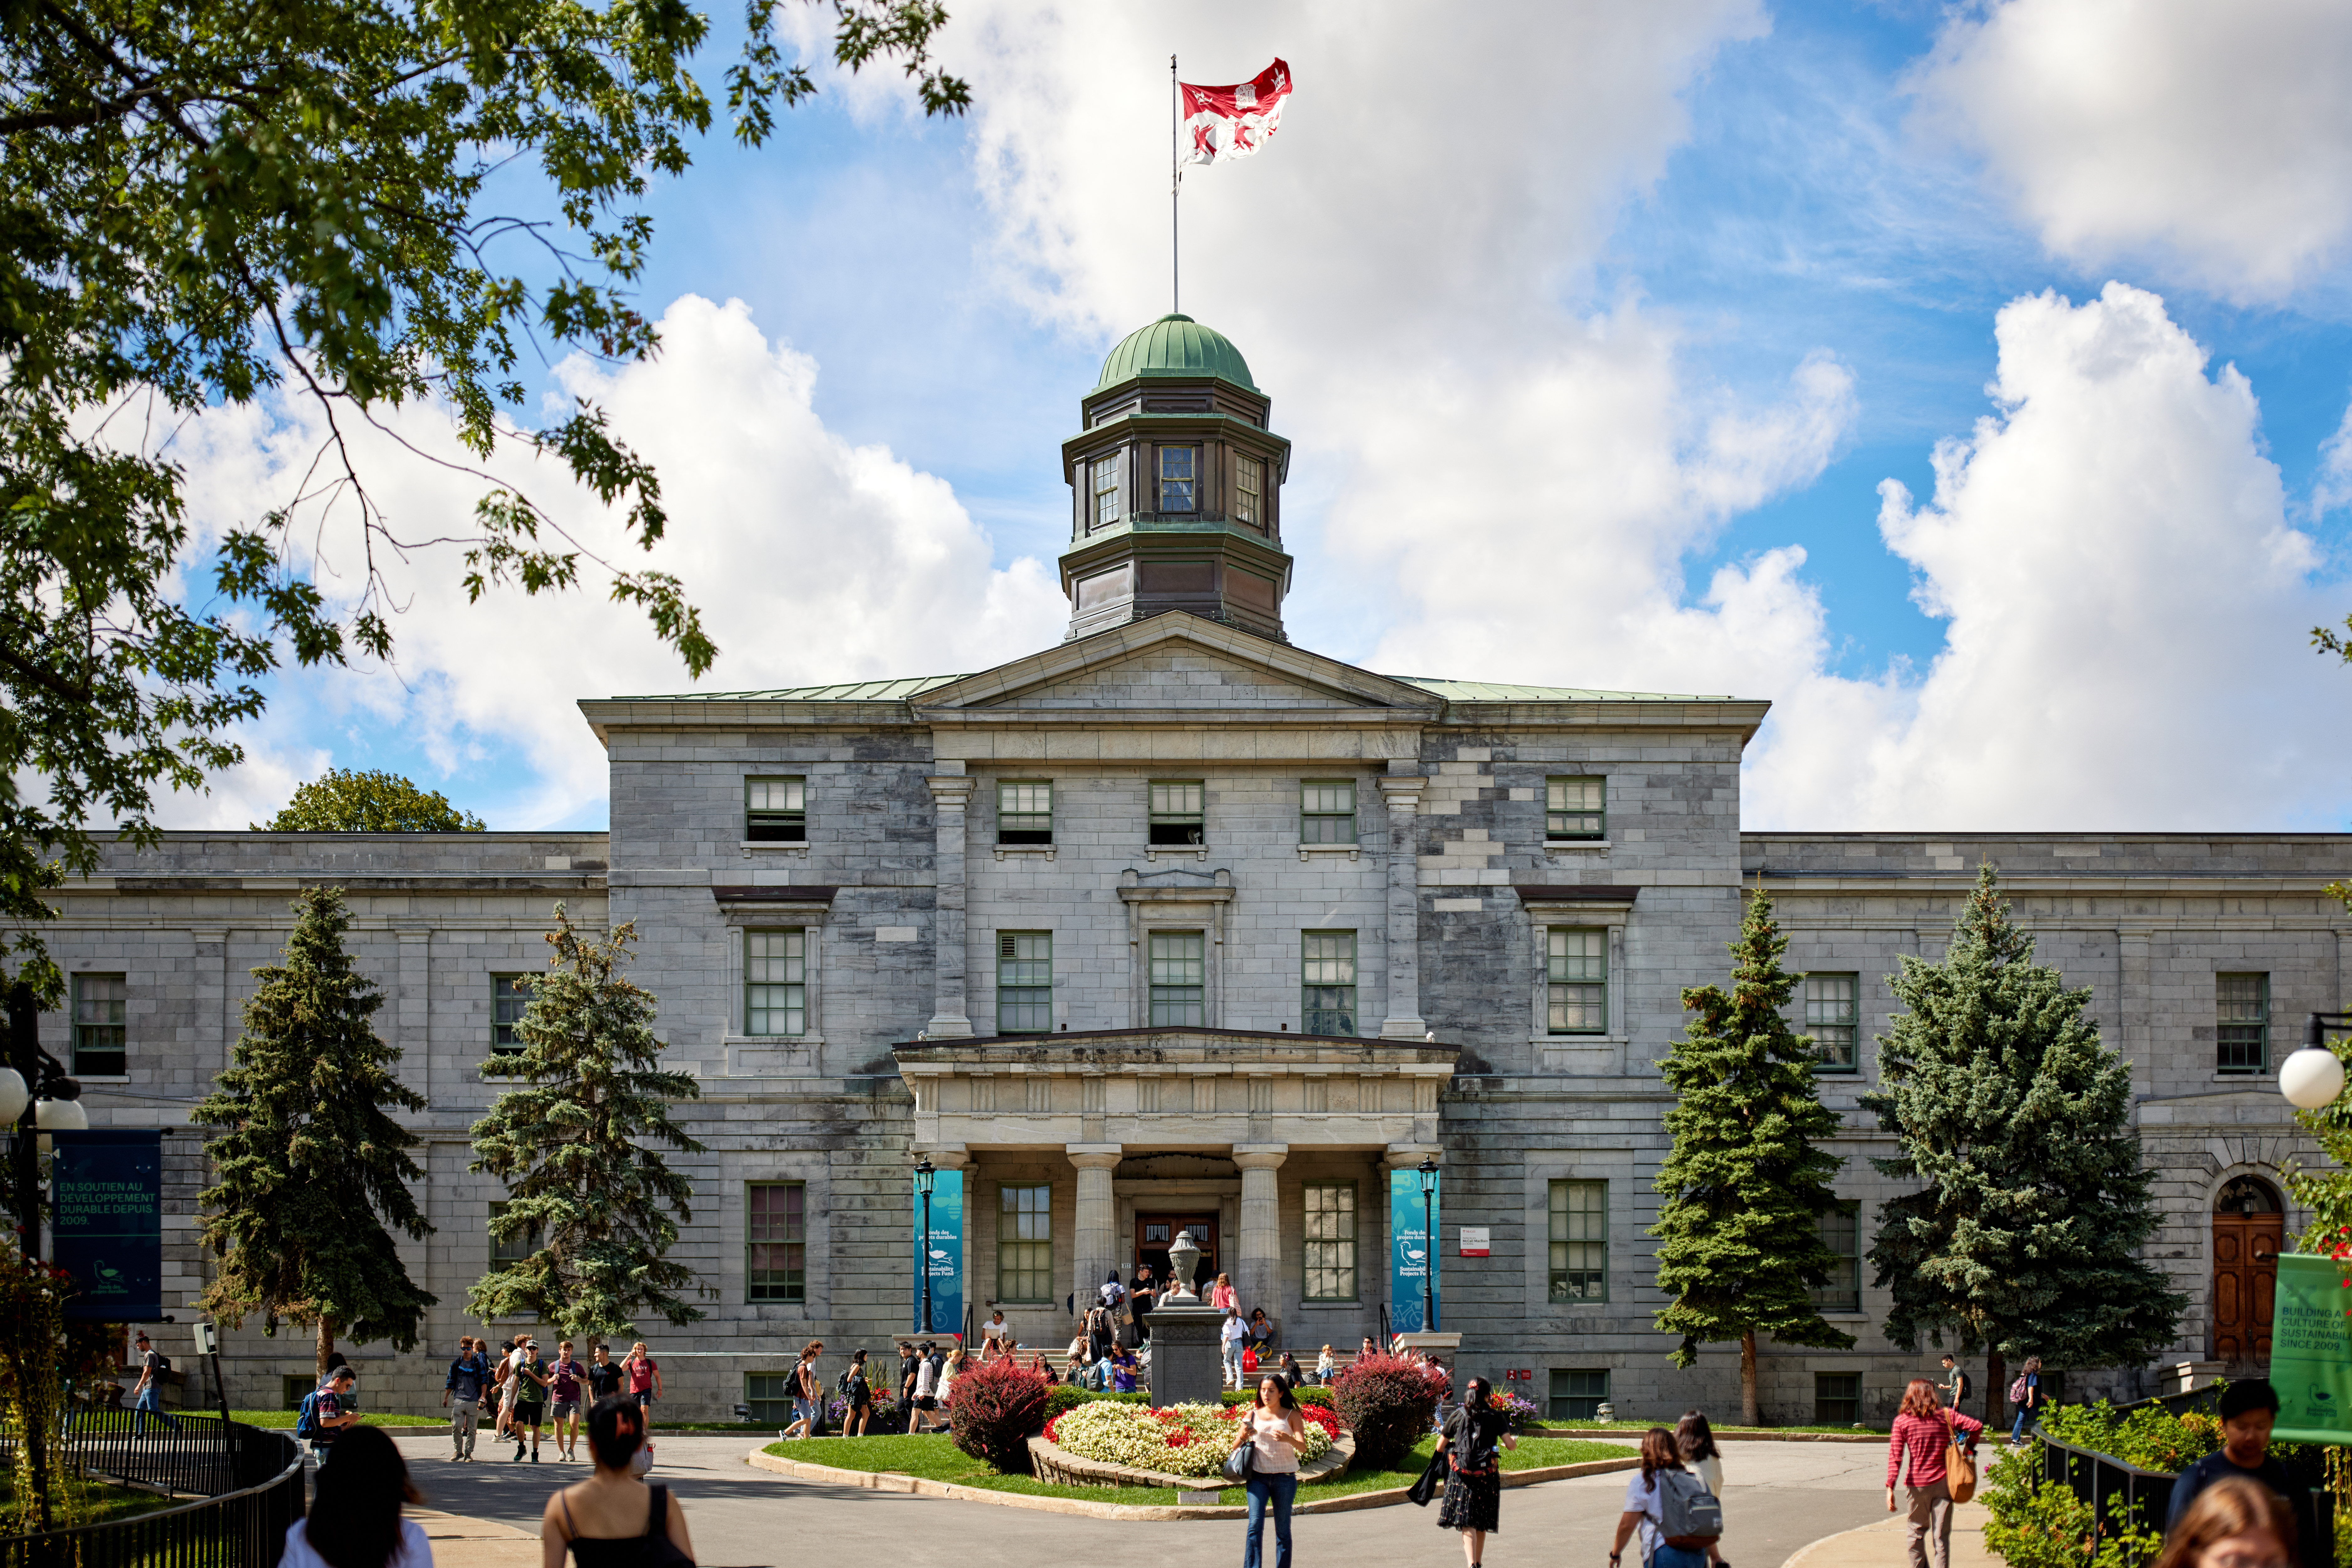
\includegraphics[scale = 0.1]{mcgill}
  \caption{Sample figure caption.}
\end{figure}


All artwork must be neat, clean, and legible. Lines should be dark enough for
purposes of reproduction. The figure number and caption always appear after the
figure. Place one line space before the figure caption and one line space after
the figure. The figure caption should be lower case (except for first word and
proper nouns); figures are numbered consecutively.


You may use color figures.  However, it is best for the figure captions and the
paper body to be legible if the paper is printed in either black/white or in
color.


\subsection{Tables}


All tables must be centered, neat, clean and legible.  The table number and
title always appear before the table.  See Table~\ref{sample-table}.


Place one line space before the table title, one line space after the
table title, and one line space after the table. The table title must
be lower case (except for first word and proper nouns); tables are
numbered consecutively.


Note that publication-quality tables \emph{do not contain vertical rules.} We
strongly suggest the use of the \verb+booktabs+ package, which allows for
typesetting high-quality, professional tables:
\begin{center}
  \url{https://www.ctan.org/pkg/booktabs}
\end{center}
This package was used to typeset Table~\ref{sample-table}.


\begin{table}
  \caption{Sample table title}
  \label{sample-table}
  \centering
  \begin{tabular}{lll}
    \toprule
    \multicolumn{2}{c}{Part}                   \\
    \cmidrule(r){1-2}
    Name     & Description     & Size ($\mu$m) \\
    \midrule
    Dendrite & Input terminal  & $\sim$100     \\
    Axon     & Output terminal & $\sim$10      \\
    Soma     & Cell body       & up to $10^6$  \\
    \bottomrule
  \end{tabular}
\end{table}

\section{Math}
If you want to write math inline text, you can use \$ $\hdots$ \$. For
example, $\lim_{x \to 0} x^2 = 0$. To write an equation on its own
line, you can use a variety of things. See below for examples:

\begin{equation} \label{eq: improblem2} 
\min_x \quad \| Kx-b \|^2_2 + \delta_S(x) + \gamma \|Dx \|_{\text{iso}}. 
\end{equation}

By adding the ``label'', you can reference it in text with such
as...Using \eqref{eq: improblem2}, we get that...

If you don't want the numbering, you can use
\begin{equation*} 
\min_x \quad \| Kx-b \|^2_2 + \delta_S(x) + \gamma \|Dx \|_{\text{iso}}. 
\end{equation*}
The ``*'' indicates that you don't want it to be numbered. It is
general practice to add numbers.

I am also going to include the .tex for the project description so
that you can see other math symbols used. 

\section{Final instructions}


Do not change any aspects of the formatting parameters in the style files.  In
particular, do not modify the width or length of the rectangle the text should
fit into, and do not change font sizes (except perhaps in the
\textbf{References} section; see below). Please note that pages should be
numbered.


\section{Preparing PDF files}


Please prepare submission files with paper size ``US Letter,'' and not, for
example, ``A4.''


Fonts were the main cause of problems in the past years. Your PDF file must only
contain Type 1 or Embedded TrueType fonts. Here are a few instructions to
achieve this.


\begin{itemize}


\item You should directly generate PDF files using \verb+pdflatex+.


\item You can check which fonts a PDF files uses.  In Acrobat Reader, select the
  menu Files$>$Document Properties$>$Fonts and select Show All Fonts. You can
  also use the program \verb+pdffonts+ which comes with \verb+xpdf+ and is
  available out-of-the-box on most Linux machines.


\item The IEEE has recommendations for generating PDF files whose fonts are also
  acceptable for NeurIPS. Please see
  \url{http://www.emfield.org/icuwb2010/downloads/IEEE-PDF-SpecV32.pdf}


\item \verb+xfig+ "patterned" shapes are implemented with bitmap fonts.  Use
  "solid" shapes instead.


\item The \verb+\bbold+ package almost always uses bitmap fonts.  You should use
  the equivalent AMS Fonts:
\begin{verbatim}
   \usepackage{amsfonts}
\end{verbatim}
followed by, e.g., \verb+\mathbb{R}+, \verb+\mathbb{N}+, or \verb+\mathbb{C}+
for $\mathbb{R}$, $\mathbb{N}$ or $\mathbb{C}$.  You can also use the following
workaround for reals, natural and complex:
\begin{verbatim}
   \newcommand{\RR}{I\!\!R} %real numbers
   \newcommand{\Nat}{I\!\!N} %natural numbers
   \newcommand{\CC}{I\!\!\!\!C} %complex numbers
\end{verbatim}
Note that \verb+amsfonts+ is automatically loaded by the \verb+amssymb+ package.


\end{itemize}


If your file contains type 3 fonts or non embedded TrueType fonts, we will ask
you to fix it.


\subsection{Margins in \LaTeX{}}


Most of the margin problems come from figures positioned by hand using
\verb+\special+ or other commands. We suggest using the command
\verb+\includegraphics+ from the \verb+graphicx+ package. Always specify the
figure width as a multiple of the line width as in the example below:
\begin{verbatim}
   \usepackage[pdftex]{graphicx} ...
   \includegraphics[width=0.8\linewidth]{myfile.pdf}
\end{verbatim}
See Section 4.4 in the graphics bundle documentation
(\url{http://mirrors.ctan.org/macros/latex/required/graphics/grfguide.pdf})


A number of width problems arise when \LaTeX{} cannot properly hyphenate a
line. Please give LaTeX hyphenation hints using the \verb+\-+ command when
necessary.

\newpage

\section*{Acknowledgments}
Please include a list of each person (with student ID) in your group
and write a paragraph \textbf{for each person} with exactly what they
did. Note that the Acknowledgment section does not count towards the
page limit.

Example Acknowledgments would look like:

\paragraph{David Hippocampus} (Student ID: 123456789) David did all
the work. He coded all the algorithms and wrote the majority of the
paper.

\paragraph{George Danzig} (Student ID: 11235712) He didn't do very
much work. Danzig was mostly focused on his other classes, namely
linear programming. 


\bibliographystyle{plainnat}
\bibliography{references.bib}

References follow the acknowledgments. Use unnumbered first-level heading for
the references. Any choice of citation style is acceptable as long as you are
consistent. It is permissible to reduce the font size to \verb+small+ (9 point)
when listing the references.
Note that the Reference section does not count towards the page limit.
\medskip



%%%%%%%%%%%%%%%%%%%%%%%%%%%%%%%%%%%%%%%%%%%%%%%%%%%%%%%%%%%%


\appendix


\section{Appendix}


Optionally include extra information (complete proofs, additional experiments and plots) in the appendix.
This section will often be part of the supplemental material.


\end{document}
